%travail_composite
\subsection{Composite}
\begin{figure}[h]
\begin{center}
    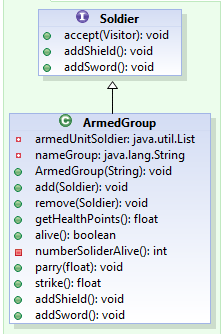
\includegraphics[width=11cm]{diagClassComposite}
\end{center}
    \caption{Diagramme de classes du pattern composite}
    \label{classes-composite}
\end{figure}

La seconde étape dans le projet consistait à rajouter la possibilité pour le client de créer des groupes armés. Un groupe armé de soldats peut être composé de plusieurs groupes armés, eux-mêmes décomposables en sous-groupes armés, et ainsi de suite. Cette notion de groupes armés fait ici apparaître une structure d'arbre avec des éléments composés d'autres éléments, structure qui fait penser à une hiérarchie. 
C'est pour cela que nous avons appliqué le pattern Composite, visible en figure \vref{classes-composite}, en créant une classe \emph{ArmedGroup} contenant une référence vers un objet \emph{Soldier} (qui représente notre \emph{procurateur}, ce que manipule le client).